\chapter{Testo del progetto}
Progettare (in breve max. 30 pagine) un sistema di prenotazione di posto a lezione, nel rispetto della (nuova) capienza delle aule (caratterizzate da un codice). La presenza degli studenti è organizzata in turni prenotabili in base alle ultime due cifre del numero di matricola (da 00 a 49 e da 50 a 99) a settimane alterne. La prenotazione per ciascun turno può essere fatta (e cancellata, per permettere a studenti in lista d’attesa di frequentare) solo dal lunedì a venerdì della settimana precedente. Al termine della prenotazione, il sistema produce una ricevuta (con aula, matricola ed orario) da scaricare/salvare. Per accedere al sistema servono le credenziali di Sapienza.\\
DA CONSEGNARE:
\begin{enumerate}
\item Analisi di contesto
\item Specifica dei requisiti
\item Analisi
\begin {enumerate}
\item[a.] Nomi/verbi
\item[b.] Schede CRC
\item[c.] Classi di analisi (stereotipi entity/boundary/control)
\item[d.] Organizzazione in package
\end{enumerate}
\item Progetto
\begin {enumerate}
\item[a.] Specifica dell’architettura
\item[b.] Classi di progetto, sottosistemi, componenti
\item[c.]  Realizzazione dei casi d’uso (sequence diagrams)
\item[d.] Cicli di vita di classi significative
\end{enumerate}
\end{enumerate}

\chapter{Analisi di contesto}


Il sistema che si vuole sviluppare si inserisce all’interno di un contesto dell’università La Sapienza di Roma  la quale ha un bacino di utenza di centinaia di migliaia di utenti tra professori, strudenti e personale interno. Il sistema di prenotazione permetterà di prenotare posti in aula comunicando con i seguenti sistemi:
\begin{itemize}
\item \textbf{Infostud}: il sistema di gestione delle tasse, voti e altre procedure di proprietà dell’università. Utile per permettere l’autenticazione tramite le credenziali già a disposizione dello studente, ottenere informazioni da usare nel sistema, come l’elenco delle lezioni e dei corsi oppure informazioni ulteriori sugli studenti.
\item Il \textbf{database delle prenotazioni}: in cui vengono conservate tutte le informazioni inerenti alle prenotaizoni (es. studente che l’ha effettuata, data, stato...).
\item Il \textbf{database delle aule}: sistema in cui sono contenute informazioni su tutte le aule in cui è possibile fare lezione quali, l’edificio in cui sono situate, il nome, la capienza, ed altre.
\end{itemize}
La figura ~\ref{figura: diagramma di contesto} riporta il diagramma di contesto  del sistema.	

\begin{figure}[htp]
\begin{center}
  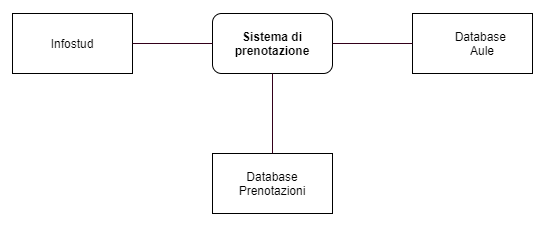
\includegraphics[width=1 \textwidth]{Figure/diagramma di contesto.png}
    \caption{Figura che mostra il dominio in cui è situato il sistema di prenotazioone.} \label{figura: diagramma di contesto}
\end{center}
\end{figure}
